\chapter{Ontwerp met Apidog}
\label{ch:apidog}

In dit hoofdstuk wordt het gebruik van \textbf{Apidog} toegelicht voor het ontwerpen van de API. Apidog maakt het mogelijk om OpenAPI-specificaties visueel op te stellen, te valideren en automatisch te documenteren, wat het ontwikkelproces gestructureerd en transparant maakt.


Met Apidog werden alle API-endpoints, datamodellen en parameters opgesteld volgens de OpenAPI-standaard. Hieronder is een voorbeeld van een datamodel in dogApi. Hieronder staan er voorbeelden van hoe het in de dogAPi er uitziet en wat het genereert.



\begin{figure}
    \centering
    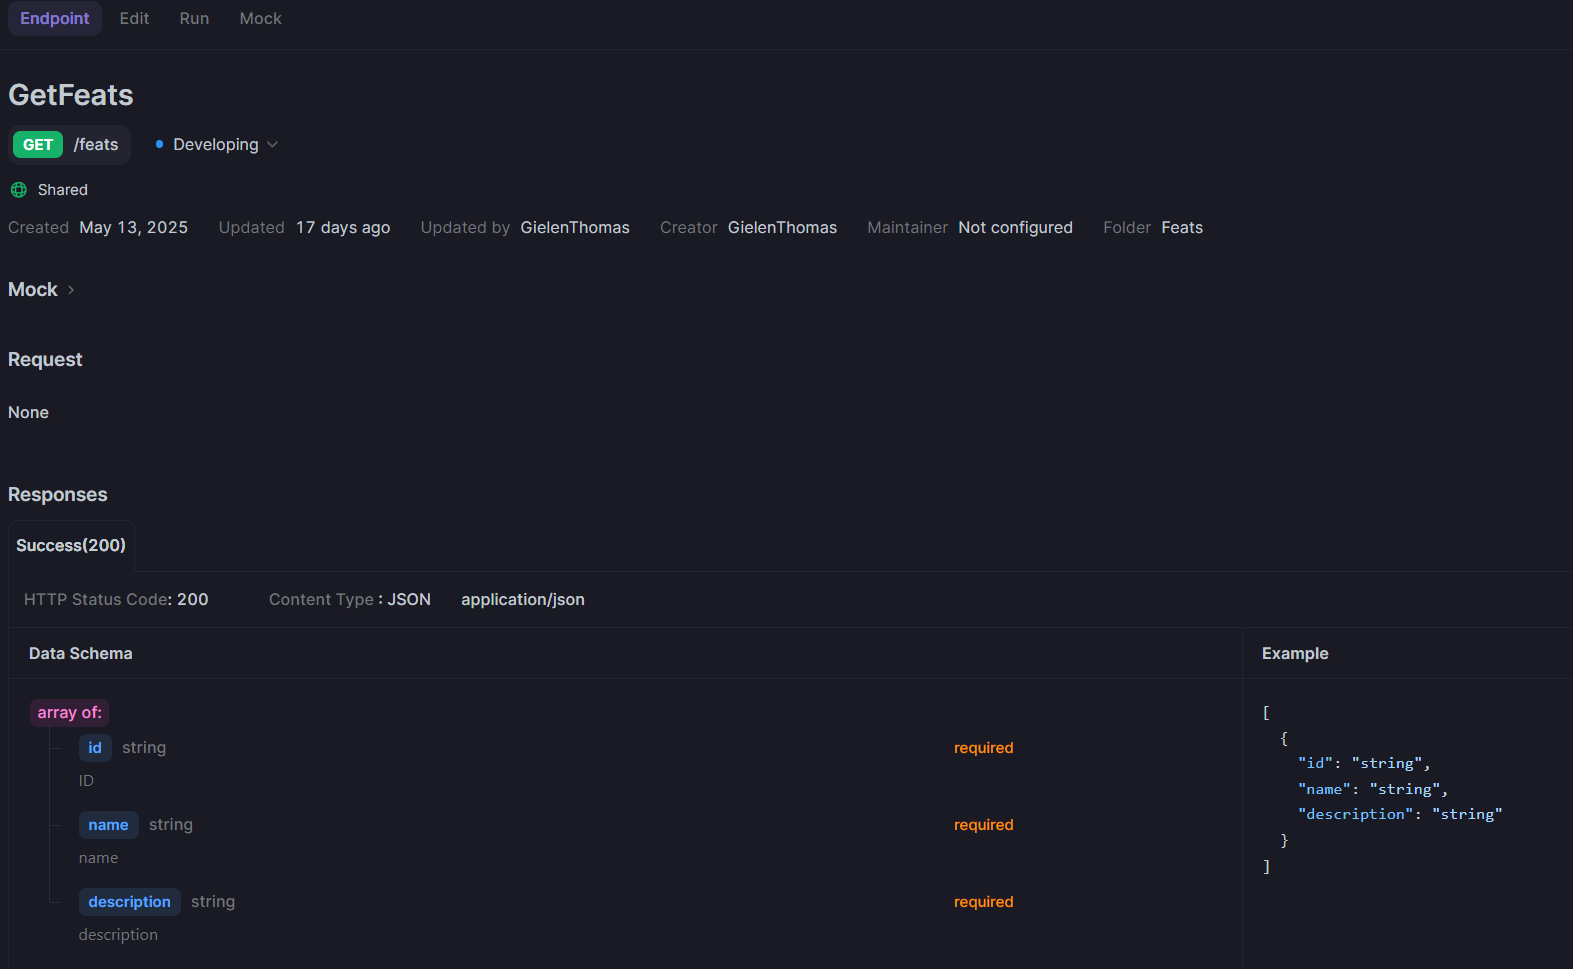
\includegraphics[width=0.8\textwidth]{end-point-voorbeeld.png}
    \caption[Voorbeeld end-point.]{\label{fig:end-point-voorbeeld}Voorbeeld van een endpoint in dogApi}
\end{figure}

\begin{listing}
    \begin{minted}{yaml}
         "/feats": {
             "get": {
                 "summary": "GetFeats",
                 "deprecated": false,
                 "description": "",
                 "tags": [],
                 "parameters": [],
                 "responses": {
                     "200": {
                         "description": "",
                         "content": {
                             "application/json": {
                                 "schema": {
                                     "type": "array",
                                     "items": {
                                         "$ref": "#/components/schemas/FeatResponse"
                                     }
                                 }
                             }
                         },
                         "headers": {}
                     }
                 },
                 "security": []
             },
    \end{minted}
    \caption[openAPIEndPoint]{End-point van de OpenAPI spec}
\end{listing}


\begin{figure}
    \centering
    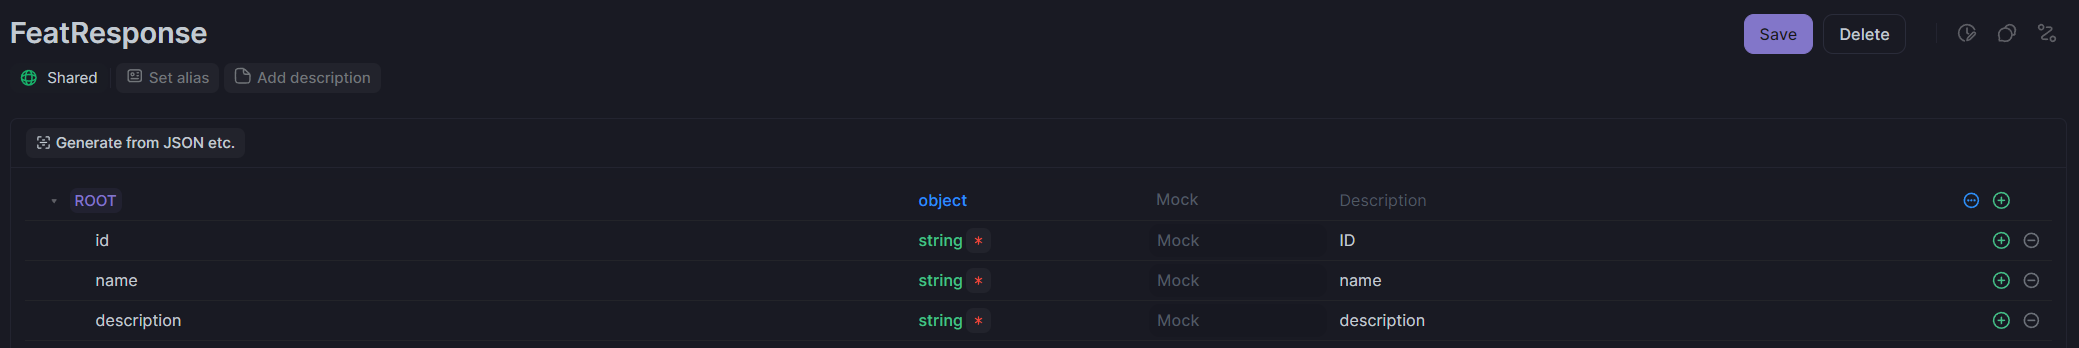
\includegraphics[width=0.8\textwidth]{data-model-voorbeeld.png}
    \caption[Voorbeeld end point.]{\label{fig:data-model-voorbeeld}Voorbeeld van een data model in dogApi}
\end{figure}

\begin{listing}
    \begin{minted}{yaml}
        "FeatResponse": {
            "type": "object",
            "properties": {
                "id": {
                    "type": "string",
                    "description": "ID"
                },
                "name": {
                    "type": "string",
                    "description": "name"
                },
                "description": {
                    "type": "string",
                    "description": "description"
                }
            },
            "required": [
            "name",
            "description",
            "id"
            ]
        },
        \end{minted}
        \caption[openAPIDataModelSpec]{Data model van de OpenApi spec}
    \end{listing}